\documentclass{beamer}
\usepackage{fontspec}
\usepackage{fontawesome}
\usepackage{hyperref}
\usetheme{metropolis}           

\title{AMSE - Präsentation}
\date{23. Oktober 2019}
\author{Benjamin Fischer}
\institute{benjamin.f.fischer@fau.de}
\begin{document}
  \maketitle

  \begin{frame}
    \frametitle{Gliederung}
    \tableofcontents
  \end{frame}

  \section{Motivation}
  
    \begin{frame}
      \frametitle{Motivation}
      \begin{itemize}
        \item Bundestag ist ein wichtiger Bestandteil der dt. Demokratie
        \item Gesetzgebung und Kontrolle der Regierungsarbeit
        \item<+-> Diskussionen und Entscheidungen über die politische Richtung 
      \end{itemize}
      \centering
      \action<+->{\textbf{Reden kommentieren, kritisieren und bewerten das politische Geschehen}}
    \end{frame}

  
  \section{Idee der App}

    \begin{frame}
      \frametitle{Grundlagen}
      \begin{itemize}
        \item App für die Darstellung von Reden im Bundestag
        \begin{itemize}
          \item Redner (Lebenslauf, Parteizugehörigkeit, etc.)
          \item Inhalt (Themen, Stichwörter, Stimmung, Zwischenrufe, etc.)
          \item Weiterführende Informationen (Nebentätigkeiten, etc.)
          \item evtl. zusätzliche Statistiken
        \end{itemize}
        \item Visuell ansprechend gestaltet
        \begin{itemize}
          \item möglichst schlicht, aber mit interessanten Zusatzinformationen
        \end{itemize}
        \item Ziel: Interesse an politischer Diskussion steigern
      \end{itemize}
    \end{frame}
  

    \begin{frame}
      \frametitle{Konzept}
      \begin{itemize}
        \item Hierarchische Navigation innerhalb der Applikation
        \begin{itemize}
          \item Bundesländer/Wahlbezirke
          \item Parteien/Listen
        \end{itemize}
        \item Anzeige der Daten für verschiedene Zeiträume 
        \begin{itemize}
          \item letzte Rede, Woche, Monat, gesamte Wahlperiode
        \end{itemize} 
        \item Zusammenfassung der Merkmale für Partei/Abgeordnete
      \end{itemize}
    \end{frame}
    
    \begin{frame}
      \frametitle{Open Data Quellen}
      \begin{itemize}
        \item Protokolle des Deutschen Bundestags
        \begin{itemize}
          \item Werden als XML-Datei bereitgestellt
          \item Dokumentation der DTD
          \item \url{https://www.bundestag.de/services/opendata}
        \end{itemize}
        \item Informationen über Parlament/Abgeordnete
        \begin{itemize}
          \item Portal des Vereins \textit{Parlamentwatch e.V.}
          \item öffentliche JSON-API (kurze Dokumentation)
          \item \url{https://www.abgeordnetenwatch.de/api}
        \end{itemize}
      \end{itemize}
    \end{frame}

    \begin{frame}
      \frametitle{Skizzen}
      \centering
      Navigation bzw. Hierarchie
      \vspace{1cm}
      \centering
      \begin{figure}[h!]
        \centering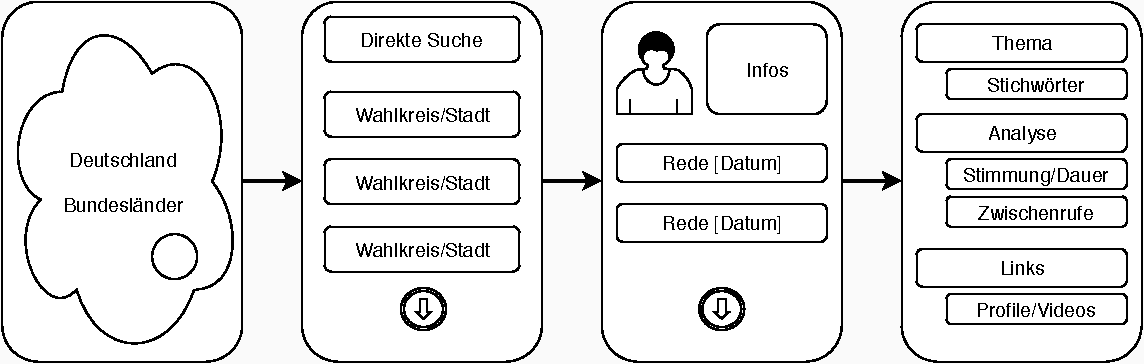
\includegraphics[width=\textwidth]{fig/mockup1.pdf}
      \end{figure}
    \end{frame}

    \begin{frame}
      \frametitle{Skizzen}
      \centering
      Hauptmenü und beispielhafte Übersicht einer Partei
      \vspace{1cm}
      \centering
      \begin{figure}[h!]
        \centering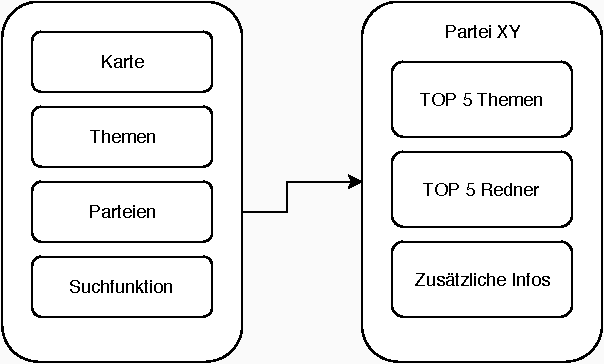
\includegraphics[width=0.6\textwidth]{fig/mockup2.pdf}
      \end{figure}
    \end{frame}


  \section{Technisches Konzept}
    \begin{frame}
      \frametitle{Überblick}
      \centering
      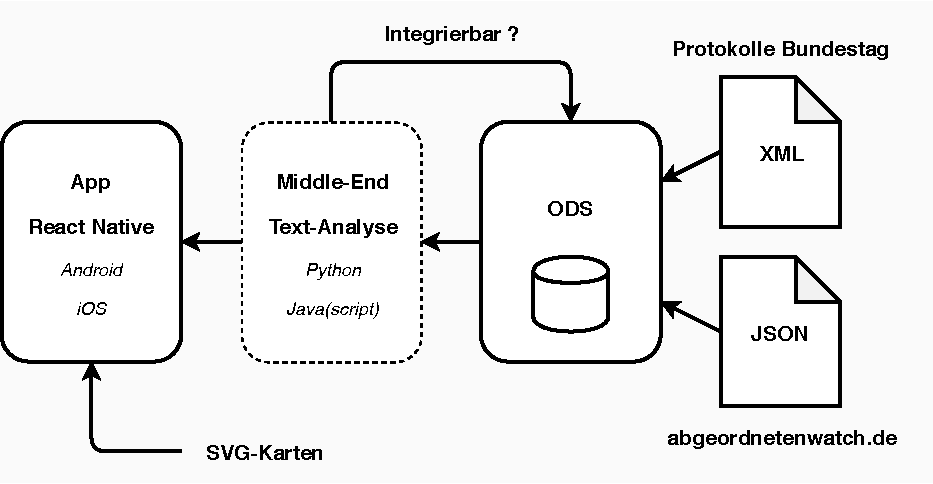
\includegraphics[width=\textwidth]{fig/tech.pdf}
    \end{frame}

    \begin{frame}
      \frametitle{Software}
      \begin{itemize}
        \item Applikation $\rightarrow$ React Native\footnote{\url{https://facebook.github.io/react-native/}} $\rightarrow$ Javascript
        \begin{itemize}
          \item Native Apps für Android/iOS
        \end{itemize}
        \item Middle-End für Textverarbeitung (nötig?) 
        \begin{itemize}
          \item Python $\rightarrow$ \textit{textblob}
          \item Java $\rightarrow$ \textit{OpenNLP}?
        \end{itemize}
        \item OpenDataService
        \begin{itemize}
          \item Anbindung beider Quellen an den ODS
          \item Ablage verarbeiteter Reden in Datenbank
        \end{itemize}
        \item Entwicklung der Services mithilfe von Docker
      \end{itemize}
    \end{frame}
  

\end{document}